\documentclass[11pt]{article}
\usepackage{amssymb}
\usepackage{amsmath, amscd}
\usepackage{changepage}
%\usepackage{fullpage}
\usepackage{parskip}
\usepackage{graphicx}
\usepackage{enumitem}
\usepackage{multicol}
\usepackage{ragged2e}
\usepackage{subfig} %Figure into table 
\usepackage{float} %Figure wrap
\usepackage{stmaryrd} %Maps from
\usepackage{sectsty}
\usepackage{setspace}
\usepackage[makeroom]{cancel}
\usepackage{environ}
\usepackage{tikz}
\usepackage{fancyhdr}
\usepackage{color}
\usepackage{framed}
\usepackage{listings}
\usepackage{hyperref}
\usepackage[left=1in, right=1in, top=1in, bottom=1in]{geometry}
%\pagestyle{fancy}
\setlength\parindent{0pt}
\allowdisplaybreaks
\input xy 
\xyoption{all}
%\allsectionsfont{\centering}

%%% HEADER, FOOTER %%%
\fancyhead{}
\lhead{Title}
\chead{}
\rhead{Page: \thepage}
%\renewcommand{\footrulewidth}{0.4pt}
\renewcommand{\headrulewidth}{0.4pt}

%%% FORMATING %%%
\newcommand{\itab}[1]{\hspace{0em}\rlap{#1}}
\newcommand{\tab}[2]{\hspace{#2\textwidth}\rlap{#1}}
\newcommand\movein[2]{\begin{adjustwidth}{#1cm}{}#2\end{adjustwidth}}

%%% MATH %%%
\newcommand\set[1]{\left\{#1\right\}}
\newcommand\bracket[1]{\left(#1\right)}
\newcommand\sqbracket[1]{\left[#1\right]}
\newcommand\norm[1]{\left\|#1\right\|}
\newcommand\abs[1]{\left|#1\right|}
\newcommand\ip[1]{\left\langle#1\right\rangle}
\newcommand\ep{\hfill$\square$}
\newcommand\real{\mathbb{R}}
\newcommand\ints{\mathbb{Z}}
\newcommand\complex{\mathbb{C}}
\newcommand\e{\mathbb{E}}
\newcommand\var{\text{Var}}

%%% TITLES %%%
\newcommand\defn{\textbf{Definition. }}
\newcommand\thm{\textbf{Theorem. }}
\newcommand\eg{\textbf{Example. }}
\newcommand\ex{\textbf{Exercise. }}
\newcommand\cor{\textbf{Corollary. }}
\newcommand\pf{\textit{Proof. }}
\newcommand\rmk{\textit{Remark. }}
\newcommand\prop{\textbf{Proposition. }}

%%% COLOURS %%%
\definecolor{dkgreen}{rgb}{0,0.6,0}
\definecolor{gray}{rgb}{0.5,0.5,0.5}
\definecolor{mauve}{rgb}{0.58,0,0.82}
\definecolor{bananamania}{rgb}{0.98, 0.91, 0.71}
\definecolor{mycolor}{rgb}{0.96,0.96,0.96}
\definecolor{gr}{rgb}{0,0,0.2}

%%% SPACE, UNDERLINE, ARROW %%%
\newcommand{\vsp}[1]{\vspace{#1ex}}
\newcommand{\ddu}[1]{\underline{\underline{#1}}}
\newcommand{\hsp}{\-\ \hspace{1ex}}

\makeatletter
\newcommand{\xRightarrow}[2][]{\ext@arrow 0359\Rightarrowfill@{#1}{#2}}
\makeatother

%%% BOXES %%%
\newcommand\centerbox[2]{
\begin{center}
\fbox   {\begin{minipage} {#1 in} \vspace{1ex}
        \begin{center} #2 \vspace{1ex}  \end{center}
        \end{minipage}
        }
\end{center}}

\newcommand\rightbox[2]{
\fbox   {\begin{minipage}{#1 in} \vspace{1ex}
            #2  \vspace{1ex}
        \end{minipage}
        }
        }

\newcommand\clrbox[1]{
\fcolorbox{gray}{mycolor}   {\begin{minipage}[t]{1.0\textwidth}
                            #1   
                            \end{minipage}
                            }
                            }
                            
\NewEnviron{elaboration}{\par
\begin{tikzpicture}
\node[rectangle,minimum width=1\textwidth] (m) {\begin{minipage}{1\textwidth}\BODY\end{minipage}};
\draw[dashed] (m.south west) rectangle (m.north east);
\end{tikzpicture}
}

\NewEnviron{elaboration2}{\par
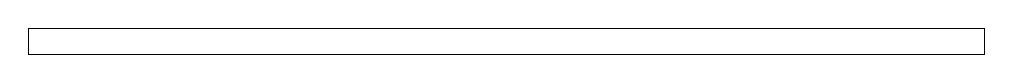
\begin{tikzpicture}
\node[rectangle,minimum width=1\textwidth] (m) {\begin{minipage}{1\textwidth}\BODY\end{minipage}};
\draw[solid] (m.south west) rectangle (m.north east);
\end{tikzpicture}
}

%%% TABLES %%%
\usepackage{array}
\newcolumntype{L}[1]{>{\raggedright\let\newline\\\arraybackslash\hspace{0pt}}m{#1}}
\newcolumntype{C}[1]{>{\centering\let\newline\\\arraybackslash\hspace{0pt}}m{#1}}
\newcolumntype{R}[1]{>{\raggedleft\let\newline\\\arraybackslash\hspace{0pt}}m{#1}}

\newcommand\tableproof[6]{
    \centering
    \begin{tabular} { C{#1cm}  C{#2cm}  C{#3cm}}
                        #4 & #5 & #6 \\
    \end{tabular}
    \justifying
}

%%% CODE %%%
\lstset{frame=single,
  backgroundcolor=\color{bananamania},
  language=Java,
  aboveskip=3mm,
  belowskip=3mm,
  showstringspaces=false,
  columns=flexible,
  numbers=left,
  basicstyle={\small\ttfamily},
  numberstyle=\tiny\color{gray},
  keywordstyle=\color{blue},
  commentstyle=\color{dkgreen},
  stringstyle=\color{mauve},
  breaklines=true,
  breakatwhitespace=true,
  tabsize=3
}

%%% LINKS %%%
\hypersetup{
    colorlinks,
    citecolor=black,
    filecolor=black,
    linkcolor=black,
    urlcolor=black
}

%%%%%%%%%%%%%%%%%%%%%%%%%%%%%%%%%%
\title{\textbf{{\vspace{-10ex}}}}
\author{\vspace{-10ex}}
\date{\vspace{-10ex}}

\begin{document}
\abovedisplayskip=5pt
\belowdisplayskip=5pt

\begin{center}
{\Large\textbf{Chevrotain: A Conflict-free Replicated Data Type Key-Value Store}}
\end{center}

\section{Introduction}
In distributed systems there is always the tension between maintaining consistency and demonstrating high performance. On one end of the spectrum there is strong consistency which implies that the distributed system behaves like a single machine that serializes all operations. Strong consistency maintains perfect data consistency at all times, at the expense of high latency due to the need for synchronization and constant communication between nodes. On the other end of the spectrum is eventual consistency which allows for states of the distributed replicas to temporarily diverge and meet later in time. Eventual consistency results in a lower frequency of communication which leads to better performance; however, eventual consistency could lead to data inconsistencies and data loss [1].

Some of the recent research focused on trying to strike a balance between strong consistency and high performance. This has led to emergence of mixed consistency semantics, such as RedBlue consistency, consistency rationing, PSI and Horus [1, 2, 3, 4]. In such semantics, strong consistency is used with operations that depend on data to be immediately consistent, while weak consistency is used with operations for which a high degree of consistency is not necessary. An alternate approach is for programmers to design the distributed system in a way that doesn’t require strong consistency at all. This is the approach that is used in concept of conflict-free replicated data types (CRDT) [5], which is the focus of this study.

In CRDTs, the distributed system is designed such that either the states of replicas could be merged in a conflict-free way at any point in time (state-based RDT or CvRDT) or that any updates to the states of the replicas are only done in a conflict-free way (op-based RDT or CmRDT) [5]. The goal of this project is to build and evaluate Chevrotain, a CRDT-based key-value store, using Golang. Both, the CvRDT and CmRDT approaches will be studied. A distributed web crawler and a mock-up network node status system will be used for evaluation.

\newpage
\section{Background}
\subsection{State-Based Convergent Replicated Data Types (CvRDT)}
In state-based replication, each update that is executed at a replica modifies the state of that replica. Then, occasionally, every replica broadcasts its local state to the other replicas, which merge the received state into its own [5].

The precise terminology is a bit complex, but for the merges to be conflict-free, the states of replicas must resemble a monotonic semilattice object. A monotonic semilattice is a term from mathematical set theory [10] but in the context of CRDTs it means the following [5]:
\begin{itemize}
 \item there is a partial order that could be used to order the states,
 \item the merge operation computes the least upper bound of the two states, and
 \item the states are monotonically non-decreasing across updates (as in the state that follows an update is ordered after the state that precedes the update).
\end{itemize}

As mentioned, the merge operation must determine something called the least upper bound of the local and incoming state. The least upper bound (or join) is yet another term from set theory [11], but it essentially means that the merge operation determines the maximal state of the local and incoming state.

The original work on CRDTs [5] provides some examples of what determining maximal state during the merge might look like. The classical example is vector clocks where the merge method takes the maximum of each respective entry. Another classical example provided by Shapiro et. all is concerned with merging logs: the merge method just takes the union of the local and incoming log.

A key-value store could be represented using sets: a set of keys and a set of values for each key. When working with sets in the CRDT framework, one approach to conflict-free merges is LWW-Element-Set (Last-Write-Wins-Element-Set). For any set, two sets are maintained: an “add set” and a “remove set”. Elements are removed from the LWW-Element-Set by being added to the remove set. All removals and additions are marked with timestamps. An element is a member of the LWW-Element-Set if it is a member of the add set and is either not in the remove set, or is in the remove set but is marked with an earlier timestamp than in the add set. In the case when the timestamps in the add and remove sets are identical, a user-defined bias towards either the add or the remove operations comes into play. Merging two replicas of the LWW-Element-Sets consist of taking the union of the respective add and remove sets [12, 13].

\subsection{Op-Based Commutative Replicated Data Types (CmRDT)}
Another approach to CRDTs is operation-based. Instead of having replicas occasionally send state to each other, whenever an update is executed at some replica, that update gets propagated to other replicas using a casual broadcasting communication protocol (CBCAST). Then there are two possible scenarios:
\begin{itemize}
\item either the updates are ordered by CBCAST and are executed in that order at each replica, or
\item the updates appear to be concurrent.
\end{itemize}

In the first scenario there are no issues and no conflicts. Now, if the updates appear to be concurrent, then one of the following approaches must take place:
\begin{itemize}
 \item the update operations are commutative (as in, the order in which they are applied at each replica is irrelevant and either order results in the same final state), or
 \item one of the update operations must be delayed until a certain pre-condition has been met, or
 \item some other approach must be used to allow the concurrent update operations to proceed.
\end{itemize}

It is not the case by all means that all of operations are commutative and Shapiro et. all do not prefer the second approach as it violates the goal of asynchrony [5]. Therefore, the third approach will be undertaken in Chevrotain, and the LWW-Element-Set approach will be used to resolve conflicts in the CmRDT implementation as well. Specifics are to follow in section 3.2.

\newpage
\section{Design} %Implementation %Execution/System Model

\newpage
\section{Evaluation}

\newpage
\section{Related Work}
There are several excellent CRDT libraries, most of them are written in JavaScript [6]. Most of those are domain specific and not directly related to key-value stores, such as the auto-merge library for JSON files [7]. When it comes to Golang, it seems there are just two implementations of CRDT in Golang: one is quite elementary [8] and the other is specific to blockchain type applications [9]. So, it is believed that this study will have at least some degree of novelty. Moreover, one the goals of this study is to compare the CvRDT and CmRDT implementations. Nevertheless, the JavaScript implementation of the auto-merge JSON library [6] and the simple CRDT Golang implementation [8] will be examined for curiosity sake and reference if need be.

\newpage
\section{Future Work}

\newpage
\section{Conclusion}

\newpage
\section*{References}

\end{document}
